
\documentclass[11pt,twoside]{article}
\usepackage{asp2010}

\resetcounters

\bibliographystyle{asp2010}

\markboth{Lubow and Budavari}{Hubble Source Catalog}

\begin{document}

\title{Hubble Source Catalog}
\author{Stephen Lubow$^1$, Tamas Budavari$^2$
\affil{$^1$Space Telescope Science Institute, 3700 San Martin Drive, Baltimore MD 21218}
\affil{$^2$Department of Physics and Astronomy, Johns Hopkins University, Baltimore MD 21218}
}

\begin{abstract}
We have created an initial catalog of objects observed by the WFPC2 and ACS instruments on the Hubble Space Telescope (HST). The catalog is based on observations taken on more than 6000 visits (telescope pointings) of ACS/WFC and more than 25000 visits of WFPC2. The catalog is obtained by cross matching by position in the sky all Hubble Legacy Archive (HLA) Source Extractor source lists for these instruments. The source lists describe properties of source detections within a visit. The calculations are performed on a SQL Server database system. First we collect overlapping images into groups, e.g., Eta Car, and determine nearby (approximately matching) pairs of sources from different images within each group. We then apply a novel algorithm for improving the cross matching of pairs of sources by adjusting the astrometry of the images. Next, we combine pairwise matches into maximal sets of possible multi-source matches. 
We apply a greedy Bayesian method to split the maximal matches into more reliable matches. We test the accuracy of the matches by comparing the fluxes of the matched sources. The result is a set of information that ties together multiple observations of the same object. A biproduct of the catalog is greatly improved relative astrometry for many of the HST images. We also provide information on nondetections that can be used to determine dropouts. With the catalog, for the first time, one can carry out time domain, multi-wavelength studies across a large set of HST data. The catalog is publicly available. Much more can be done to expand the catalog capabilities.

\end{abstract}

\section{Source Lists}

The Hubble Legacy Archive (HLA) provides source lists,
lists of sources detected by HST \cite{2008ASPC..394..481W}. To obtain these source lists,
first color combined ("white-light") images within a visit are produced for
each detector to obtain the deepest possible image.
Second, for each detected source, the individual color images 
are searched to detect the source at the position indicated by the white-light image
and to determine its properties.
The source list determinations are carried out using Source Extractor
and DOAPhot software. There is then for each visit, a Source Extractor and DAOPhot source list of detected
sources in each color and detector appropriate to that visit.
 The source lists contain positional information about each
source, together with photometeric and other source properties. 
These source lists provide the basic input data to the Hubble Source Catalog (HSC).
The current version of the HSC uses Source Extractor
source lists only for WFPC2 and ACS/WFC images.

\section{Image Grouping}
To perform the cross matching for the HSC, we first group all images
being considered (ACS/WFC and WFPC2) into maximal groups of overlapping
images.  These image groups are constructed by applying the friend-of-friends
algorithm to images, where a friend is required to overlap with some image
in the group to some threshold value, currently set to 10\% of the WFPC2 aperture area.
The grouping effectively partitions the set of source lists being cross matched into
disjoint subsets that can be more analyzed for efficiently for cross matches.

\section{Pairwise Matching}

We determine nearby pairs of sources across source lists within the same image group.
A certain cutoff threshold is applied in making this pairing determination.
The set of paired sources is stored in the database.

\section{Astrometric Correction}

The next step is to bring the overlapping images into better alignment, that is,
improve the relative astrometric accuracy of the images in each group.
This process involves adjusting the astrometry of each
image within an image group so as to  minimize the sum of the separations of the
pairs of nearby sources involving that image described in the previous section.
To carry out this step, we have devised a new algorithm that is based
on applying 3D rotations on the images. 
For small astrometric corrections,
the effect of applying a 3D rotation can be simply expressed in terms
of a cross product involving the position vector on the unit sphere
with the 3D rotation vector. A key step in the minimization process involves adjusting
the astrometry of
each image within a group, while regarding all other images as having fixed astrometry.
For small (infinitestimal) adjustments in astrometry of each image, the minimization of the residual astrometric errors
has an analytic solution
that involves the inversion of a $3 \times 3$ matrix \cite{2012arXiv1206.0644B}. This analytic solution allows the astrometric correction to be applied
 in a fast and efficient manner. The astrometric correction (3D rotation)
for every image within the group is corrected in this way. After determining the corrections
to all images within the group, we apply the corrections  to all
sources in the group. This process of correcting the astrometry of all sources in the group
is iterated multiple (currently 50) times.
In carrying out these corrections, not all image pairs are considered. After carrying out
half the iterations, a certain threshold on pairwise separations %(currently 0.1 arc-sec) 
is applied
to eliminate false pairs. Only pairs that satisfy that threshold are considered in  subsequent
iterations of the astrometric correction process.

\section{Cross Matching}
Having obtained the astrometrically corrected source lists, we then determine which
sets of sources match together. That is, we are determining which sources describe
the same astronomical object, across visits, filters, images, and detectors. 
This determination is an inherently statistical decision.
To carry out this process, we first determine a new list of source pairs, based on 
the updated astrometry, subject to a cutoff threshold. %that is currently set to 0.1 arc-sec. 
We then apply 
a friends-of-friends algorithm to construct maximal sets of matching objects.
These maximal sets can sometimes produce chains whose endpoints
may be far apart and thus should not not part of the same match. To correct this situation,
we developed a tool called the {\it chainbreaker} that considers various partitionings
of these maximal sets using a greedy algorithm. We
compute a Bayes factor for each partitioning based on \cite{2008ApJ...679..301B} that takes into account
the inherent positional uncertainty of each source position. The partitioning with
the highest value of the Bayes factor (most probable) is regarded as describing the sources
that match together. In most cases, the favored match is the original one determined
by the friends-of-friends algorithm, i.e., not involving further partitioning.. 

\section{Catalog}
We construct a database table that describes each source. Each source in a match has the same matchid value.
Sources with the same matchid value are considered to be describing the same astronomical
object. The catalog includes all sources in the source lists, even if they do not match
another source (singletons). Sources that are not well detected (HLA flag values greater than 4)
are included in the table but marked as nondetections. The table is searched by position (ra, dec,
and search radius) by means of
a SQL server table valued function.  Searching takes advantage of HTM indexing
on the position of each source and is very fast.
This function has an option to provide a list of WFPC2 and ACS images for which no source detection
lies within the search radius. In this way, all color source detections, dropouts, and image
nondetections are provided by the search function.  There are currently, about 45 million
source detections and 15 million color dropouts in the catalog.

There are currently two forms based interfaces to the catalog that follow
the conventions of MAST. The forms are available through \url{http://archtest.stsci.edu/hst/hla_cat/}.
The detailed form allows users to obtain information as a table with one row per source.
The information includes the corrected position and magnitude of each source., as well as the position
of each match.
The other form, called the summary form, allows users to obtain information as a table with one row per match.
On this form one obtains the position of each match and the average magnitude of the sources
in each match in several filters.

\section{Results}


The code for the catalog consists  of scripts that contain SQL statements
and call SQL stored procedures and user defined SQL functions.
The code that carries out the astrometric corrections and matching includes  C\# functions that are
embedded in the database through DLLs as extended stored procedures. The generation of the catalog
takes a few days  with SQL Server 2008 running on a single (aging) Dell PowerEdge 2950 server with 
Intel Xeon E5430 @ 2.66Ghz (2 processors) and 24GB of memory.

The HSC has produced improved astrometry for about half the WFPC2 and ACS/WFC
images. 
Typically, the improvements are greater than a factor of 3 reduction in relative positional errors across overlapping
images.
In some cases, an order of magnitude improvement was made.
%There are a few major factors that limit the number of images that can be corrected.
%First, about 20\% of these images did not have source lists, likely due to problems with the images
%themselves. About 40\% of the images with source lists were not astrometrically corrected.
%In addition, about 60\% of these images without corrections did not overlap with other images and therefore
%could could be corrected. 
In some other cases, images could not be corrected because
the image offsets were larger than was assumed in our current tool or did not have enough sources in common 
with another image. We have started experimenting
with using larger threshold parameters for matching pairs.

Another issue is the quality of matches created by our current procedure.
The current set of parameters for producing matches is quite conservative
and results in a small fraction of sources that are erroneously matched. We estimate the number
such cases by looking at the distribution of fluxes for pairs of sources in the same
match that have the same filter and detector. These flux differences are typically only a few
percent. We find that there is only a small
fraction of cases with large flux differences.  We therefore conclude that only a small fraction
of the matches contain sources that do not belong together in the match. On
the other hand, we find that there are cases of nearby matches that have similar
fluxes in the same filter. This indicates that such matches should be merged together.
This result suggests that some adjustments to the matching parameters/algorithm would be useful.

More details on the algorithms and results are found in \cite{2012arXiv1206.0644B}.

We have been examining the discovery potential of the catalog. 
We have been analyzing cases where pairs of sources with the same filter and detector
within a match have undergone substantial flux variations in time. A small fraction of objects ($\la 0.1 \%$)
have flux variations by more than a factor of 2. In some cases, these    objects correspond
to known GRBs and supernovae (see Fig 1).  In other cases, we have found problems with
the images or source lists. We then may be able to identify and prune/correct problem
images. Other cases appear to be previously unknown variable objects.
In addition, the catalog may provide a useful role as a tool to examine the long term trends
in the HST performance.


\begin{figure}
\centering
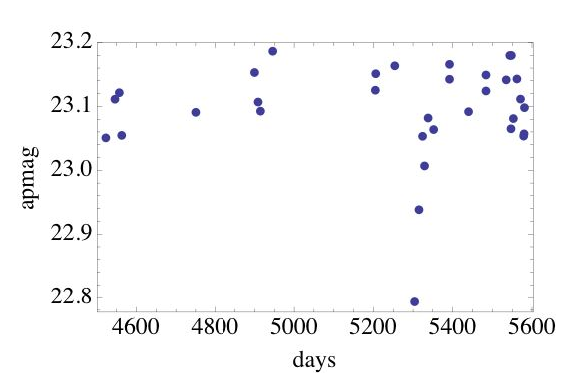
\includegraphics[width=6.0cm]{O21_1.eps}
\caption{Aperture magnitude in filter F850LP for ACS/WFC 
as a function of time in days since Jan. 1 , 1990 for a HSC match that contains 
the distant ($Z> 1$) supernova Thames.}
\end{figure}


\acknowledgements We acknowledge support from NASA AISRP grant NNX09AK62.

\bibliography{O21}


\end{document}
